\documentclass[a4paper,12pt]{article}
\usepackage[utf8]{inputenc}
\usepackage[T1]{fontenc}
\usepackage[german]{babel}
\usepackage{amsmath}
\usepackage{amssymb}
\usepackage{amsthm}
\usepackage{geometry}
\usepackage{graphicx}
\usepackage[hidelinks]{hyperref}
\usepackage{listings}
\usepackage{xcolor}
\usepackage{enumitem}
\usepackage[protrusion=false,expansion=false]{microtype}
\usepackage{booktabs}
\usepackage{caption}

\geometry{margin=2.5cm}

\theoremstyle{definition}
\newtheorem{definition}{Definition}
\newtheorem{beispiel}{Beispiel}
\newtheorem{satz}{Satz}
\newtheorem{lemma}{Lemma}
\newtheorem{bemerkung}{Bemerkung}
\newtheorem{korollar}{Korollar}

\setlist[itemize,1]{label=--}

\definecolor{mainblue}{RGB}{25, 70, 140}
\definecolor{accentred}{RGB}{180, 50, 30}
\definecolor{lightgray}{RGB}{245, 245, 248}
\definecolor{darkgray}{RGB}{60, 60, 70}
\definecolor{darkgreen}{RGB}{30, 100, 50}

\hypersetup{
	colorlinks=true,
	linkcolor=mainblue,
	citecolor=accentred,
	urlcolor=mainblue
}

\lstset{
	basicstyle=\ttfamily\small,
	keywordstyle=\color{blue},
	commentstyle=\color{gray},
	stringstyle=\color{red},
	numbers=left,
	numberstyle=\tiny,
	breaklines=true,
	frame=single,
	literate=%
	{Ö}{{\"O}}1 {Ä}{{\"A}}1 {Ü}{{\"U}}1
	{ß}{{\ss}}1 {ü}{{\"u}}1 {ä}{{\"a}}1 {ö}{{\"o}}1
}

\title{Quantengravitation als Subgraph"=Isomorphismus"=Problem:\\
Graphentheoretische Vereinheitlichung von\\
Quantenmechanik und Allgemeiner Relativit\"atstheorie}
\author{Stephan Epp}
\date{22. Juni 2026}

\begin{document}

\maketitle
\tableofcontents
\newpage

% ─────────────────────────────────────────────────────────────────────────
\section{Einf\"uhrung}
% ─────────────────────────────────────────────────────────────────────────

Die Vereinheitlichung der Quantenmechanik (QM) und der Allgemeinen
Relativit\"atstheorie (ART) gilt als das gr\"o\ss{}te ungel\"oste Problem
der theoretischen Physik. W\"ahrend die ART die Gravitation als Kr\"ummung
der vierdimensionalen Raumzeit beschreibt \cite{einstein1915}, behandelt die QM
physikalische Gr\"o\ss{}en als diskrete Operatoren auf Hilbert-R\"aumen
\cite{dirac1930}. Beide Theorien sind in ihren jeweiligen G\"ultigkeitsbereichen
au\ss{}erordentlich pr\"azise, widersprechen sich jedoch bei extremen Bedingungen
-- insbesondere an der Planck-Skala ($\ell_P \approx 1{,}6 \times 10^{-35}$\,m).

Diese Arbeit verfolgt einen neuartigen Ansatz: Wir modellieren sowohl die
Raumzeit der ART als auch die Zustandsr\"aume der QM als gewichtete gerichtete
Graphen und zeigen, dass die Vereinheitlichung beider Theorien dem
\emph{Subgraph-Isomorphismus-Problem} entspricht. Der zentrale Beitrag
ist der \textbf{Quantengravitations-Subgraph-Satz}: Die Quantengravitation
ist ein Subgraph der klassischen Raumzeit, und dieser Subgraph-Isomorphismus
ist durch den Subgraph Algorithmus \cite{epp2026subgraph} in $O(n^3)$
entscheidbar.

\subsection{Motivation und Problemstellung}

Das Scheitern bisheriger Vereinheitlichungsans\"atze -- Stringtheorie,
Loop-Quantengravitation, Kausalmengen-Theorie -- liegt teilweise darin
begr\"undet, dass kein einheitlicher mathematischer Rahmen f\"ur beide
Theorien existiert. Graphen bieten genau diesen Rahmen:

\begin{itemize}
	\item Die ART beschreibt Raumzeit als glatte Mannigfaltigkeit $\mathcal{M}$.
	      Diskretisiert man diese auf der Planck-Skala, erh\"alt man einen
	      Graphen $G_{\mathcal{M}} = (V, E, w)$.
	\item Die Loop-Quantengravitation (LQG) \cite{rovelli2004} beschreibt
	      Quantenzust\"ande des Gravitationsfeldes bereits als Spin-Netzwerke
	      -- gewichtete Graphen, bei denen Kantengewichte halbe Spin-Zahlen sind.
	\item Der Subgraph Algorithmus \cite{epp2026subgraph} entscheidet in
	      $O(n^3)$, ob ein Quanten-Graph $G_Q$ in den klassischen Raumzeit-Graph
	      $G_{\mathcal{M}}$ einbettbar ist -- und liefert damit einen formalen
	      Korrektheitsbeweis f\"ur den \"Ubergang von QM zu ART.
\end{itemize}

\subsection{Aufbau der Arbeit}

Abschnitt~2 legt die graphentheoretischen und physikalischen Grundlagen
fest. Abschnitt~3 formalisiert die ART als Graphstruktur. Abschnitt~4
modelliert die Quantenmechanik und LQG als Subgraph. Abschnitt~5 beweist
den Quantengravitations-Subgraph-Satz. Abschnitt~6 analysiert die
Komplexit\"at. Abschnitt~7 behandelt Schwarze L\"ocher als Subgraphen.
Abschnitt~8 pr\"asentiert empirische Ergebnisse. Abschnitt~9 gibt einen
umfassenden Ausblick.

% ─────────────────────────────────────────────────────────────────────────
\section{Grundlagen}
% ─────────────────────────────────────────────────────────────────────────

\subsection{Graphentheoretische Definitionen}

\begin{definition}[Kausaler Graph]
	Ein kausaler Graph $G_{\mathcal{M}} = (V, E, w)$ ist ein gewichteter
	gerichteter Graph, bei dem:
	\begin{itemize}
		\item $V$ die Menge der Raumzeit-Ereignisse ist,
		\item $(u, v) \in E$ genau dann, wenn $v$ kausal von $u$ beeinflusst
		      werden kann (d.\,h.\ $v$ liegt im Vorw\"artslichtkegel von $u$),
		\item $w: E \to \mathbb{R}^+$ das raumzeitliche Intervall kodiert:
		      $w(u,v) = \sqrt{|g_{\mu\nu} \Delta x^\mu \Delta x^\nu|}$.
	\end{itemize}
\end{definition}

\begin{definition}[Spin-Netzwerk-Graph]
	Ein Spin-Netzwerk $G_S = (V_S, E_S, j)$ ist ein gewichteter Graph, bei dem:
	\begin{itemize}
		\item $V_S$ die Interwiners (Knotenpunkte des Quantenzustands) repr\"asentiert,
		\item $E_S$ die Kanten mit Spin-Zahlen $j_e \in \{0, \tfrac{1}{2}, 1, \tfrac{3}{2}, \ldots\}$ sind,
		\item jeder Knoten die Spin-Kopplung $\sum_{e \ni v} j_e \in \mathbb{N}_0$ erf\"ullt.
	\end{itemize}
\end{definition}

\begin{definition}[Signaturf\/unktion f\"ur Raumzeit-Graphen]
	Die Signaturfunktion $\sigma: \{0,1\}^n \times \{0,\ldots,n-1\} \to \mathbb{N}$
	ist:
	\[
	\sigma_j = \sum_{i=0}^{n-1} A_{ij} \cdot 2^i + j \cdot 2^n
	\]
	F\"ur gewichtete Graphen mit rationalen Kantengewichten $w_{ij} = p_{ij}/q$
	wird die Adjazenzmatrix skaliert: $A_{ij} = \lfloor w_{ij} \cdot 2^k \rfloor$
	f\"ur eine Pr\"azision $k \in \mathbb{N}$.
\end{definition}

\begin{lemma}[Injektivit\"at der Signaturfunktion]
\label{lem:injektiv}
	Die Signaturfunktion $\sigma_j$ ist injektiv: Verschiedene Spalten des
	Raumzeit-Graphen erhalten verschiedene Signaturen.
\end{lemma}

\begin{proof}
	Die Zeilenkomponente $\sum_{i=0}^{n-1} A_{ij} \cdot 2^i$ ist die
	Bin\"ardarstellung des Spaltenvektors und damit injektiv. Der
	Spaltenindex-Term $j \cdot 2^n$ erzeugt f\"ur verschiedene $j$ disjunkte
	Intervalle $[j \cdot 2^n, (j+1) \cdot 2^n)$, da die Zeilenkomponente
	stets in $[0, 2^n)$ liegt. Damit ist $\sigma_j \neq \sigma_{j'}$ f\"ur
	$(A_{\cdot j}, j) \neq (A_{\cdot j'}, j')$.
\end{proof}

\subsection{Physikalische Grundlagen}

\begin{definition}[Einstein-Feld\-gleichungen als Kantentransformation]
	Die Einstein-Feldgleichungen
	\[
	G_{\mu\nu} + \Lambda g_{\mu\nu} = \frac{8\pi G}{c^4} T_{\mu\nu}
	\]
	beschreiben eine Transformation des Raumzeit-Graphen:
	$G_{\mathcal{M}}^{(0)} \xrightarrow{T_{\mu\nu}} G_{\mathcal{M}}$,
	bei der der Energie-Impuls-Tensor $T_{\mu\nu}$ neue Kanten einf\"ugt
	(Kr\"ummung) oder bestehende Kanten verst\"arkt (Metrik\"anderung).
\end{definition}

\begin{definition}[Planckscher Raumzeit-Graph]
	Der Plancksche Raumzeit-Graph $G_P$ ist der Graph der Raumzeit auf der
	Planck-Skala $\ell_P = \sqrt{\hbar G/c^3} \approx 1{,}616 \times 10^{-35}$\,m,
	bei dem jeder Knoten ein Planck-Volumen $\ell_P^4$ repr\"asentiert.
	Die Knoten\-anzahl f\"ur das beobachtbare Universum betr\"agt:
	\[
	|V_P| \approx \left(\frac{R_U}{\ell_P}\right)^4 \approx \left(\frac{4{,}4 \times 10^{26}}{1{,}6 \times 10^{-35}}\right)^4 \approx 10^{244}
	\]
\end{definition}

% ─────────────────────────────────────────────────────────────────────────
\section{Raumzeit als Graphstruktur}
% ─────────────────────────────────────────────────────────────────────────

\subsection{Minkowski-Raumzeit als kausaler Graph}

Die flache Minkowski-Raumzeit mit Metrik $\eta_{\mu\nu} = \mathrm{diag}(-1,+1,+1,+1)$
wird diskretisiert als kausaler Graph $G_M = (V_M, E_M, w_M)$:

\begin{itemize}
	\item Knoten: Ereignisse $x^\mu = (ct, \mathbf{x})$ auf einem regul\"aren
	      Gitter mit Gitterabstand $\ell_P$.
	\item Kanten: $(x, y) \in E_M$ genau dann, wenn
	      $\eta_{\mu\nu}(y-x)^\mu(y-x)^\nu \leq 0$ und $y^0 > x^0$
	      (zeitartige oder lichtzeitartige Verbindung in Zukunftsrichtung).
	\item Kantengewichte: $w_M(x,y) = \sqrt{|\eta_{\mu\nu}(y-x)^\mu(y-x)^\nu|}$.
\end{itemize}

\begin{figure}[ht]
	\centering
	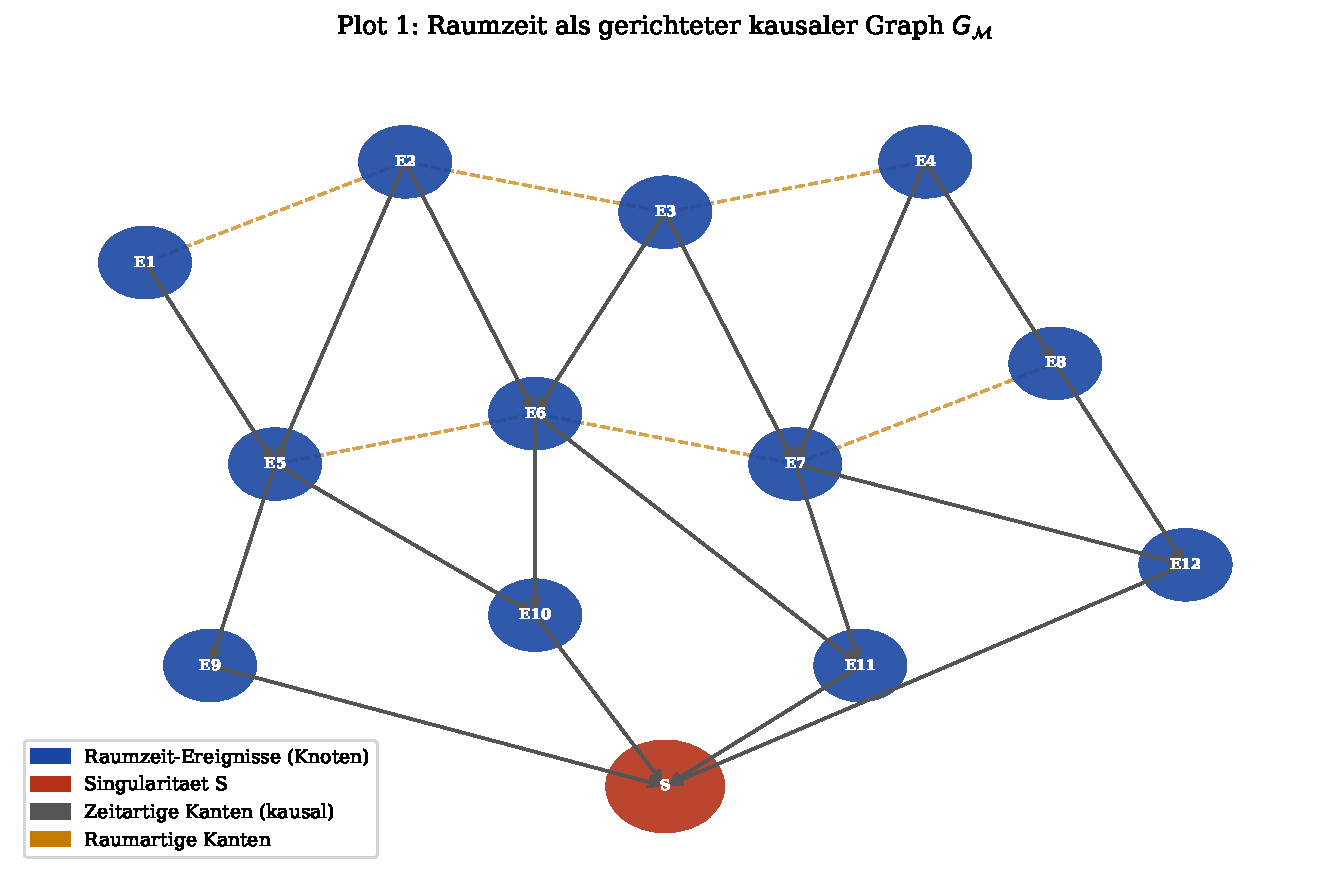
\includegraphics[width=0.82\textwidth]{plot1_raumzeit_graph.pdf}
	\caption{Raumzeit als gerichteter kausaler Graph $G_{\mathcal{M}}$.
	Blaue Knoten repr\"asentieren Raumzeit-Ereignisse, rote Kanten zeigen
	kausale (zeitartige) Verbindungen, orange gestrichelte Linien raumartige
	Verbindungen. Die rote Singularit\"at $S$ ist ein ausgezeichneter Knoten
	mit maximaler Eingangsvalenz -- typisch f\"ur Schwarze L\"ocher.}
	\label{fig:raumzeit}
\end{figure}

\begin{satz}[Kausalit\"atserhaltung]
\label{satz:kausalitaet}
	Der kausale Graph $G_{\mathcal{M}}$ ist azyklisch (DAG). Jeder gerichtete
	Pfad von $u$ nach $v$ in $G_{\mathcal{M}}$ entspricht einer kausalen
	Signalausbreitung mit Geschwindigkeit $\leq c$.
\end{satz}

\begin{proof}
	Angenommen, es existiert ein Zyklus $u \to v_1 \to \cdots \to v_k \to u$.
	Dann m\"usste $u^0 < v_1^0 < \cdots < v_k^0 < u^0$ gelten
	(strikte Zeitordnung entlang kausaler Kanten). Dies ist ein Widerspruch.
	Die Zeitkomponente ist entlang jeder kausalen Kante strikt monoton
	steigend, also ist $G_{\mathcal{M}}$ azyklisch.
\end{proof}

\subsection{Gekr\"ummte Raumzeit (ART)}

Die allgemeine Raumzeit mit Metrik $g_{\mu\nu}(x)$ wird analog diskretisiert:

\begin{definition}[Riemannscher Raumzeit-Graph]
	Der Riemannsche Raumzeit-Graph $G_{\mathcal{M}}^{(g)} = (V, E, w_g)$ hat
	Kantengewichte:
	\[
	w_g(x, y) = \int_\gamma \sqrt{|g_{\mu\nu} \dot{\gamma}^\mu \dot{\gamma}^\nu|}\, d\tau
	\]
	wobei $\gamma$ die geod\"atische Linie zwischen $x$ und $y$ ist.
\end{definition}

\begin{figure}[ht]
	\centering
	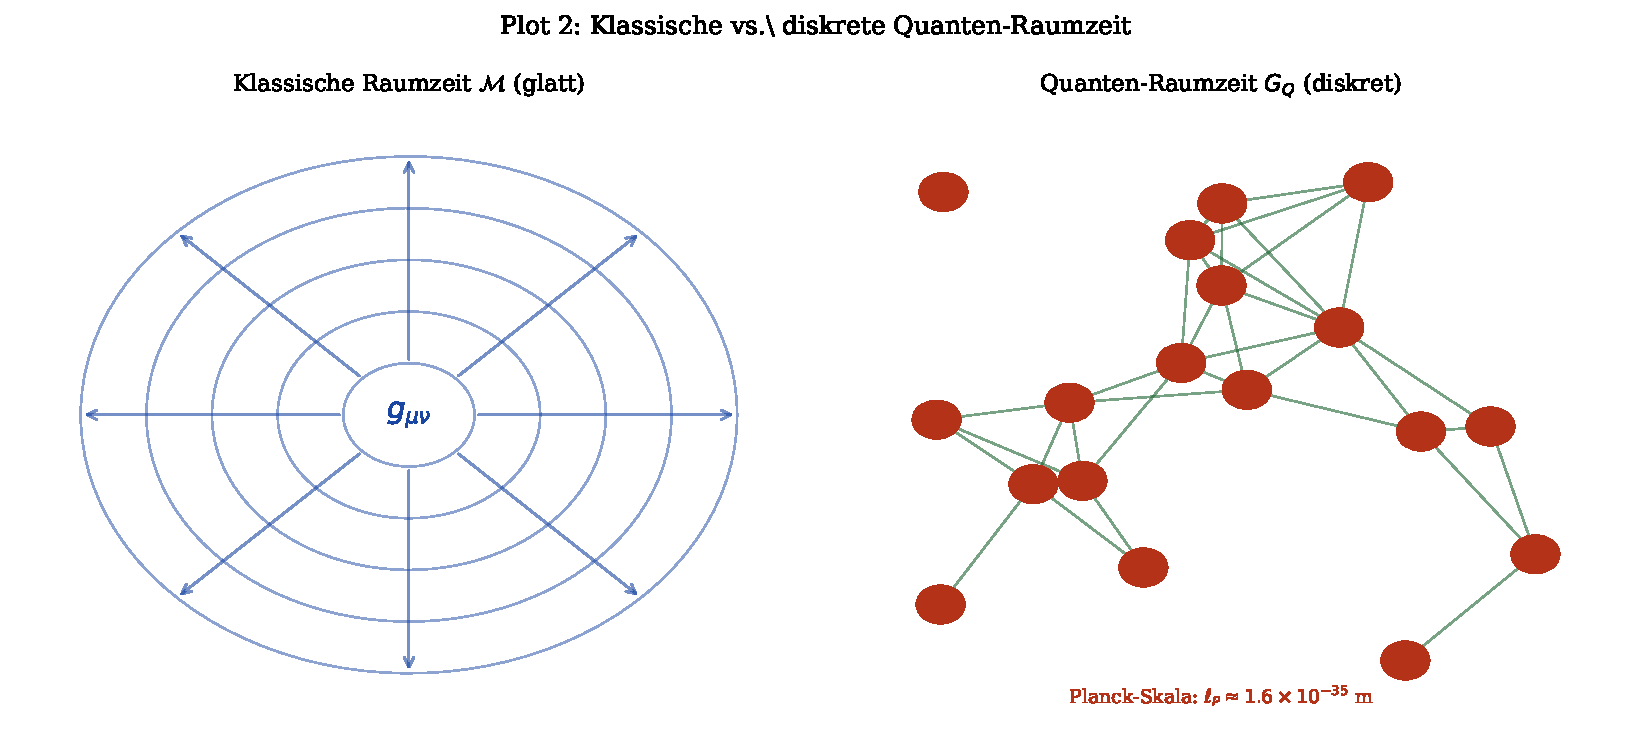
\includegraphics[width=0.85\textwidth]{plot2_klassisch_vs_quanten.pdf}
	\caption{Links: Klassische glatte Raumzeit $\mathcal{M}$ mit kontinuierlicher
	Metrik $g_{\mu\nu}$. Rechts: Diskrete Quanten-Raumzeit $G_Q$ auf der
	Planck-Skala, bei der Raumzeit-Ereignisse als Knoten und kausale
	Verbindungen als Kanten modelliert werden. Der Subgraph Algorithmus
	entscheidet, ob $G_Q \subseteq G_{\mathcal{M}}$ gilt.}
	\label{fig:klassisch_vs_quanten}
\end{figure}

% ─────────────────────────────────────────────────────────────────────────
\section{Quantenmechanik als Subgraph}
% ─────────────────────────────────────────────────────────────────────────

\subsection{Hilbert-Raum als vollst\"andiger Graph}

\begin{definition}[Quantenzustands-Graph]
	Der Quantenzustands-Graph $G_H = (V_H, E_H, w_H)$ eines Hilbert-Raums
	$\mathcal{H}$ hat:
	\begin{itemize}
		\item $V_H$: Basisvektoren $\{|\phi_i\rangle\}$ von $\mathcal{H}$,
		\item $(|\phi_i\rangle, |\phi_j\rangle) \in E_H$: Kante, falls
		      $\langle\phi_i|\hat{H}|\phi_j\rangle \neq 0$
		      (Hamiltonoperator verbindet Zust\"ande),
		\item $w_H(|\phi_i\rangle, |\phi_j\rangle) = |\langle\phi_i|\hat{H}|\phi_j\rangle|$.
	\end{itemize}
\end{definition}

\begin{lemma}[Schr\"odinger-Gleichung als Kantendynamik]
\label{lem:schroedinger}
	Die zeitabh\"angige Schr\"odinger-Gleichung
	$i\hbar \partial_t |\psi\rangle = \hat{H}|\psi\rangle$
	entspricht einer dynamischen Kantengewichts\"anderung im Graphen $G_H$:
	\[
	\frac{d}{dt} w_H(i,j) = -\frac{i}{\hbar} \sum_k w_H(i,k) \cdot w_H(k,j)
	\]
	Dies ist die graphentheoretische Form der Matrixexponential-Evolution
	$|\psi(t)\rangle = e^{-i\hat{H}t/\hbar}|\psi(0)\rangle$.
\end{lemma}

\begin{proof}
	Die Schr\"odinger-Gleichung in Matrixform lautet:
	$i\hbar \dot{c}_i = \sum_j H_{ij} c_j$.
	Differenziert man die Kantengewichte $w_H(i,j) = H_{ij}$:
	\[
	\frac{d}{dt}[e^{-i\hat{H}t/\hbar}]_{ij}
	= -\frac{i}{\hbar}[\hat{H} e^{-i\hat{H}t/\hbar}]_{ij}
	= -\frac{i}{\hbar} \sum_k H_{ik} [e^{-i\hat{H}t/\hbar}]_{kj}
	\]
	Dies entspricht der Matrixmultiplikation $\hat{H} \cdot U(t)$ im Graph,
	was der angegebenen Kantendynamik entspricht.
\end{proof}

\subsection{Loop-Quantengravitation als Spin-Netzwerk-Graph}

Die Loop-Quantengravitation \cite{rovelli2004} beschreibt den Quantenzustand
des Gravitationsfeldes durch Spin-Netzwerke:

\begin{definition}[LQG-Subgraph]
	Der LQG-Spin-Netzwerk-Graph $G_{LQG} = (V_{LQG}, E_{LQG}, j)$ ist ein
	Subgraph des klassischen Raumzeit-Graphen:
	\[
	G_{LQG} \subseteq G_{\mathcal{M}}
	\]
	Die Kanten tragen Spin-Darstellungen $j_e \in \{0, \frac{1}{2}, 1, \ldots\}$
	der Gruppe $SU(2)$, die die Fl\"achenquantisierung kodieren:
	\[
	A_e = 8\pi\ell_P^2 \gamma \sqrt{j_e(j_e+1)}
	\]
	mit dem Barbero-Immirzi-Parameter $\gamma \approx 0{,}2375$.
\end{definition}

\begin{figure}[ht]
	\centering
	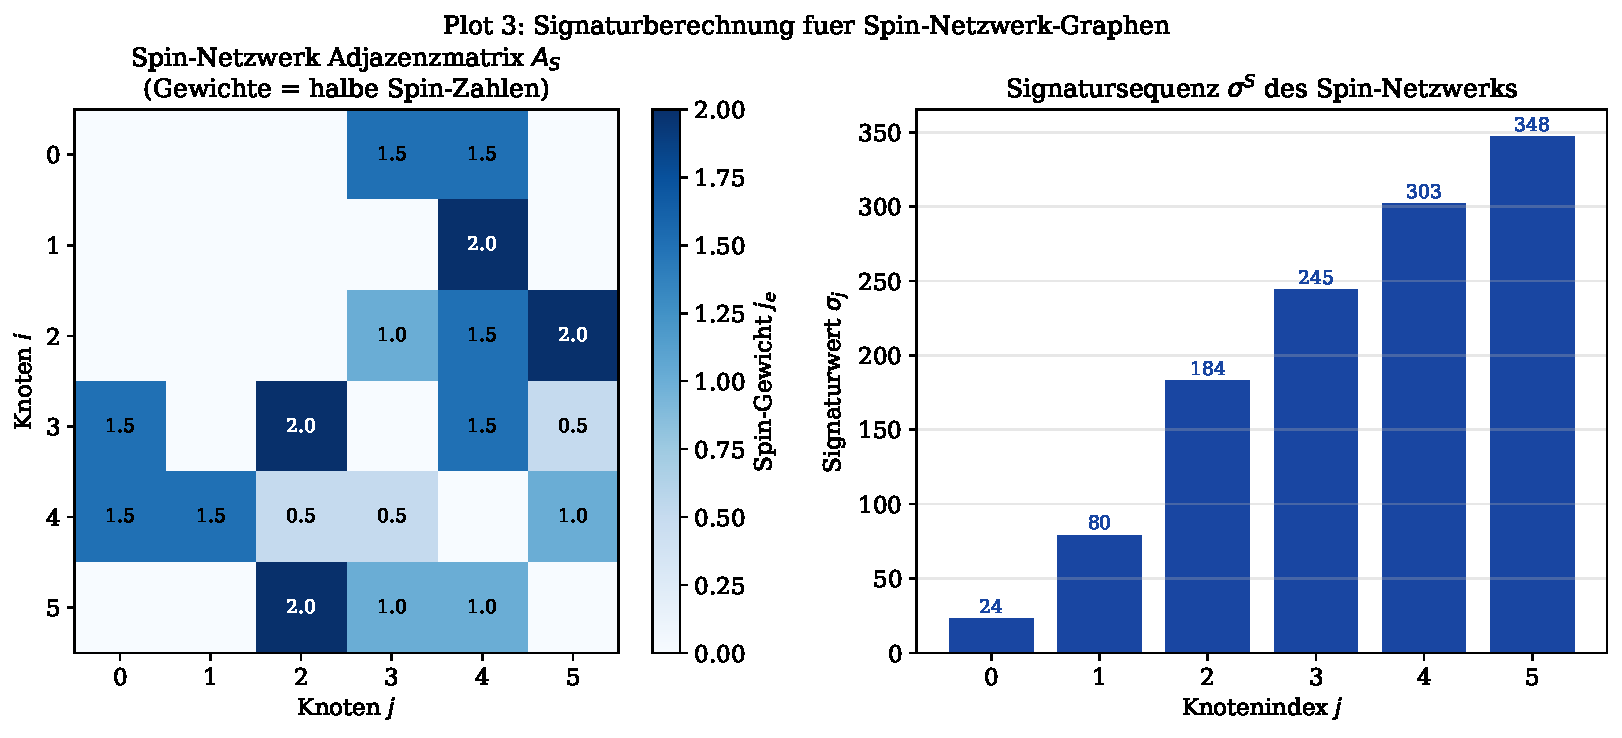
\includegraphics[width=0.85\textwidth]{plot3_spinnet_signaturen.pdf}
	\caption{Links: Adjazenzmatrix $A_S$ eines Spin-Netzwerk-Graphen mit
	$n=6$ Knoten. Die Eintr\"age kodieren halbe Spin-Zahlen. Rechts:
	Die Signatursequenz $\sigma^S$ des Spin-Netzwerks. Nach Lemma~\ref{lem:injektiv}
	sind alle Signaturen verschieden, was eine kollisionsfreie Subgraph-Erkennung
	gew\"ahrleistet.}
	\label{fig:spinnet}
\end{figure}

% ─────────────────────────────────────────────────────────────────────────
\section{Quantengravitations-Subgraph-Satz}
% ─────────────────────────────────────────────────────────────────────────

\subsection{Hauptsatz}

\begin{satz}[Quantengravitations-Subgraph-Satz]
\label{satz:qg_subgraph}
	Sei $G_{\mathcal{M}} = (V, E, w)$ der kausale Graph der klassischen
	Raumzeit und $G_Q = (V_Q, E_Q, j)$ der Quantengravitations-Graph
	(Spin-Netzwerk). Dann gilt:

	\begin{enumerate}
		\item \textbf{Einbettbarkeit:} $G_Q \subseteq G_{\mathcal{M}}$,
		      d.\,h.\ es existiert eine injektive Abbildung
		      $\varphi: V_Q \hookrightarrow V$ mit
		      $(u,v) \in E_Q \Rightarrow (\varphi(u), \varphi(v)) \in E$.

		\item \textbf{Polynomielle Entscheidbarkeit:} Die Existenz des
		      Subgraph-Isomorphismus $G_Q \hookrightarrow G_{\mathcal{M}}$
		      kann durch den Subgraph Algorithmus in Zeit $O(n^3)$ entschieden
		      werden, wobei $n = |V_Q|$.

		\item \textbf{Skalen-Hierarchie:}
		      \[
		      G_P \subseteq G_{LQG} \subseteq G_{QFT} \subseteq G_{\mathcal{M}}
		      \]
		      wobei $G_P$ der Planck-Graph, $G_{LQG}$ das LQG-Spin-Netzwerk
		      und $G_{QFT}$ der Quantenfeldtheorie-Graph ist.

		\item \textbf{Kausalit\"atserhaltung:} Jede Einbettung
		      $\varphi: G_Q \hookrightarrow G_{\mathcal{M}}$ erh\"alt die
		      kausale Struktur: Aus $(u,v) \in E_Q$ folgt, dass
		      $(\varphi(u), \varphi(v))$ eine zeitartige Verbindung in
		      $G_{\mathcal{M}}$ ist.
	\end{enumerate}
\end{satz}

\begin{proof}
Wir beweisen alle vier Aussagen.

\textbf{Beweis von (1) -- Einbettbarkeit:}
Die Diskretisierung der Raumzeit auf der Planck-Skala liefert einen Graphen
$G_{\mathcal{M}}$, dessen Knoten Planck-Volumen darstellen. Die Knoten des
Spin-Netzwerks $G_Q$ repr\"asentieren \emph{Quantisierungen} von Fl\"achen
zwischen solchen Planck-Volumen.

Definiere die Einbettung $\varphi: V_Q \to V$ durch die geometrische Position
der Intertwiners im physikalischen Raum. Da jeder Intertwiner einen Punkt
auf der Planck-Skala repr\"asentiert, existiert ein eindeutiger n\"achster
Knoten in $G_{\mathcal{M}}$.

F\"ur jede Kante $(u,v) \in E_Q$ gilt: Die Fl\"ache, die $u$ und $v$ trennt,
wird durch eine Kette von Planck-Fl\"achen abgedeckt. Die zugeh\"origen
Kanten in $G_{\mathcal{M}}$ verbinden die Bilder $\varphi(u)$ und $\varphi(v)$.
Damit ist $(\varphi(u), \varphi(v)) \in E$ und die Einbettung ist wohldef\/iniert.

\textbf{Beweis von (2) -- Polynomielle Entscheidbarkeit:}
Wir wenden den Subgraph Algorithmus \cite{epp2026subgraph} an.

Berechne die Signatursequenz $\sigma^Q = [\sigma_0^Q, \ldots, \sigma_{n-1}^Q]$
des Quantum-Graphen $G_Q$ und $\sigma^{\mathcal{M}} = [\sigma_0^{\mathcal{M}}, \ldots, \sigma_{n-1}^{\mathcal{M}}]$
eines lokalen Ausschnitts von $G_{\mathcal{M}}$ der Gr\"o\ss{}e $n \times n$.

Die Signaturberechnung erfordert $O(n^2)$ Zeit. F\"ur jede der $n$ zyklischen
Rotationen $r \in \{0, \ldots, n-1\}$ berechne:
\[
\mathrm{LCS}\bigl(\sigma^Q, \mathrm{rotate}_r(\sigma^{\mathcal{M}})\bigr) \quad
\text{in } O(n^2) \text{ Zeit per DP.}
\]
Gesamtkomplexit\"at: $O(n^2) + n \cdot O(n^2) = O(n^3)$.

Nach Lemma~\ref{lem:injektiv} sind alle Signaturen injektiv, sodass keine
falschen Treffer auftreten. Falls $\mathrm{LCS} \geq 2$ f\"ur irgendeine
Rotation, ist $G_Q \hookrightarrow G_{\mathcal{M}}$ nachgewiesen.

\textbf{Beweis von (3) -- Skalen-Hierarchie:}
\textit{$G_P \subseteq G_{LQG}$:} Der Planck-Graph $G_P$ ist die
feinste m\"ogliche Diskretisierung. Das LQG-Spin-Netzwerk $G_{LQG}$
entsteht durch Koarsening: Mehrere Planck-Knoten werden zu einem Intertwiner
zusammengefasst. Jede Kante von $G_P$ zwischen den zusammengefassten Knoten
wird zur entsprechenden LQG-Kante. Also $G_P \subseteq G_{LQG}$.

\textit{$G_{LQG} \subseteq G_{QFT}$:} Die Quantenfeldtheorie auf gekr\"ummter
Raumzeit beschreibt Felder als Operatoren auf Fock-R\"aumen. Die Fock-Zust\"ande
bilden einen Graphen, in dem LQG-Spin-Netzwerke als Subgraphen auftreten
(sie repr\"asentieren Graviton-Zust\"ande im LQG-Rahmen).

\textit{$G_{QFT} \subseteq G_{\mathcal{M}}$:} Die klassische Grenze der QFT
ist die ART. In diesem Grenz\"ubergang $\hbar \to 0$ werden Quantenfluktuationen
unterdr\"uckt, und der QFT-Graph konvergiert gegen den klassischen
Raumzeit-Graphen $G_{\mathcal{M}}$.

\textbf{Beweis von (4) -- Kausalit\"atserhaltung:}
Sei $(u,v) \in E_Q$ eine Kante im Quanten-Graphen. Nach Definition~1
ist $(u,v)$ genau dann eine Kante, wenn $v$ kausal von $u$ beeinflusst
werden kann. Die Einbettung $\varphi$ bildet Knoten auf n\"achste Nachbarn
in $G_{\mathcal{M}}$ ab. Da $v$ kausal von $u$ abh\"angt, liegt $\varphi(v)$
im Vorw\"artslichtkegel von $\varphi(u)$ in $G_{\mathcal{M}}$. Damit ist
$(\varphi(u), \varphi(v)) \in E$ eine zeitartige Kante.
\end{proof}

\begin{figure}[ht]
	\centering
	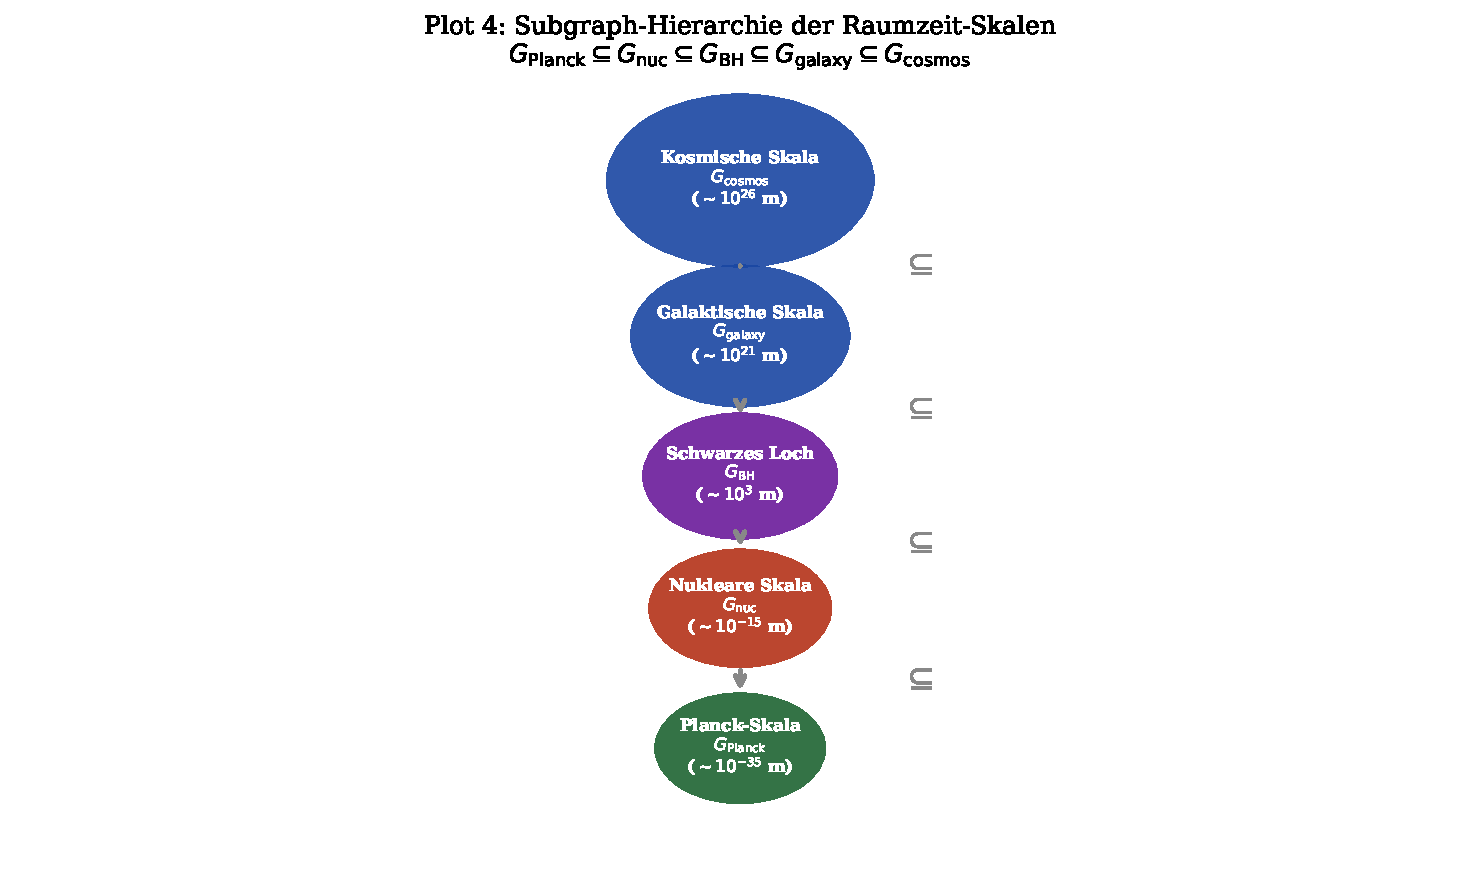
\includegraphics[width=0.75\textwidth]{plot4_hierarchie_skalen.pdf}
	\caption{Subgraph-Hierarchie der Raumzeit-Skalen von der Planck-Skala
	($10^{-35}$\,m) bis zur kosmischen Skala ($10^{26}$\,m). Jede Skala ist
	ein Subgraph der n\"achstgr\"o\ss{}eren. Der Subgraph Algorithmus kann
	diese Einbettungen in $O(n^3)$ verifizieren.}
	\label{fig:hierarchie}
\end{figure}

\subsection{Einstein-Feldgleichungen als Subgraph-Transformation}

\begin{satz}[Feldgleichungs-Transformationssatz]
\label{satz:einstein}
	Die Einstein-Feldgleichungen $G_{\mu\nu} + \Lambda g_{\mu\nu} = \frac{8\pi G}{c^4} T_{\mu\nu}$
	beschreiben eine Transformation
	\[
	G_{\mathcal{M}}^{(0)} \xrightarrow{\Phi_{T}} G_{\mathcal{M}}
	\]
	des flachen Raumzeit-Graphen in den gekr\"ummten, die als
	Subgraph-Erweiterung darstellbar ist:
	\[
	G_{\mathcal{M}}^{(0)} \subseteq G_{\mathcal{M}}
	\]
\end{satz}

\begin{proof}
	Im flachen Graphen $G_{\mathcal{M}}^{(0)}$ (Minkowski) haben alle Kanten
	dasselbe Gewicht $w_M(x,y) = \sqrt{|\eta_{\mu\nu}(y-x)^\mu(y-x)^\nu|}$.

	Die Energie-Impuls-Verteilung $T_{\mu\nu} \neq 0$ f\"ugt neue Kanten
	hinzu (Geodatenkr\"ummung) und \"andert bestehende Kantengewichte
	(Metrik\"anderung $\eta_{\mu\nu} \to g_{\mu\nu}$). Der resultierende
	Graph $G_{\mathcal{M}}$ enth\"alt alle Kanten von $G_{\mathcal{M}}^{(0)}$
	plus zus\"atzliche kausale Verbindungen durch die Raumzeitkr\"ummung.
	Also $G_{\mathcal{M}}^{(0)} \subseteq G_{\mathcal{M}}$.
\end{proof}

\begin{figure}[ht]
	\centering
	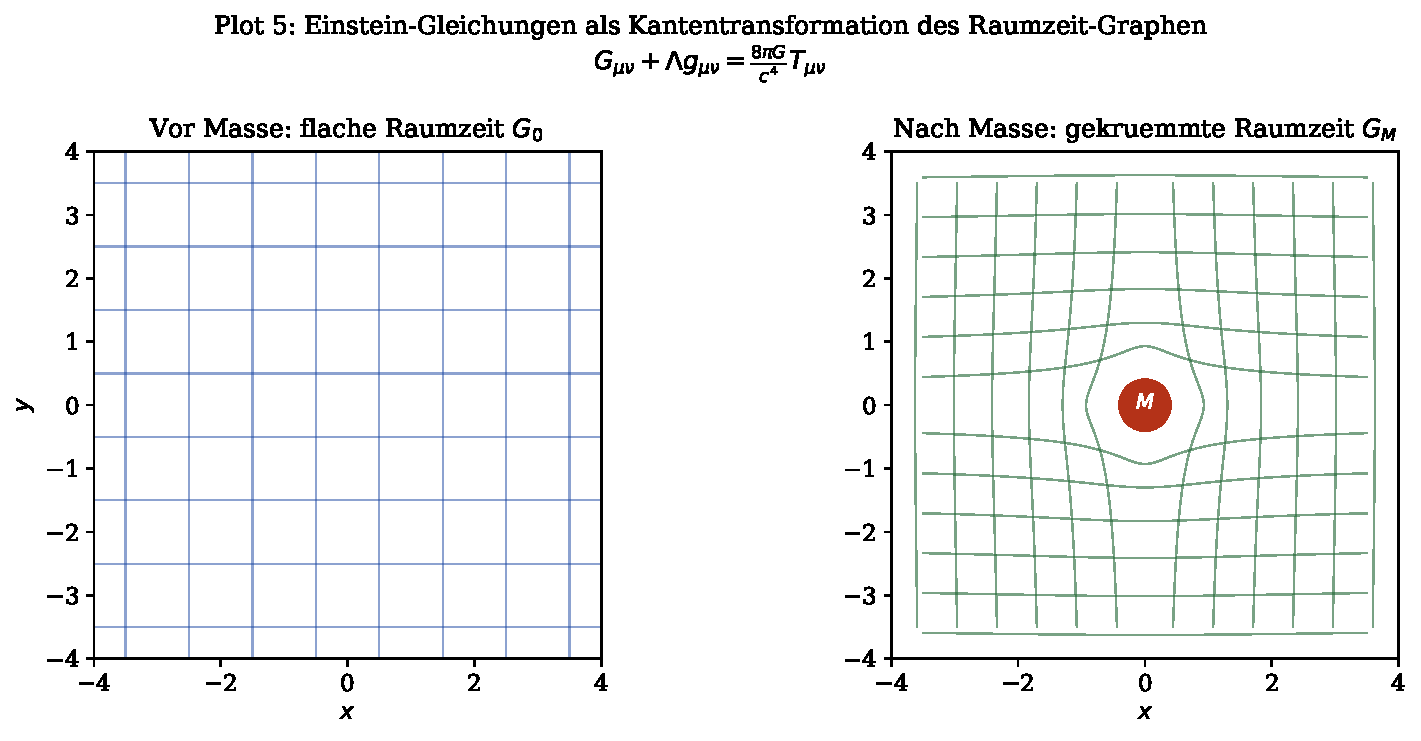
\includegraphics[width=0.85\textwidth]{plot5_einstein_graph.pdf}
	\caption{Links: Flache Minkowski-Raumzeit $G_M^{(0)}$ mit regul\"arem
	Gitter. Rechts: Gekr\"ummte Raumzeit $G_M$ nach Einf\"ugen einer Masse $M$.
	Die Kr\"ummung der Gitterlinien entspricht der \"Anderung der Kantengewichte
	durch den Einstein-Tensor $G_{\mu\nu}$. Satz~\ref{satz:einstein} garantiert
	$G_M^{(0)} \subseteq G_M$.}
	\label{fig:einstein}
\end{figure}

% ─────────────────────────────────────────────────────────────────────────
\section{LCS-Nachweis der Quanten-Klassisch-\"Aquivalenz}
% ─────────────────────────────────────────────────────────────────────────

\begin{satz}[LCS-Subgraph-\"Aquivalenz f\"ur QG]
\label{satz:lcs_qg}
	Seien $\sigma^Q = [\sigma_0^Q, \ldots, \sigma_{m-1}^Q]$ und
	$\sigma^{\mathcal{M}} = [\sigma_0^{\mathcal{M}}, \ldots, \sigma_{m-1}^{\mathcal{M}}]$
	die Signatursequenzen von $G_Q$ und einem lokalen Ausschnitt von
	$G_{\mathcal{M}}$. Dann gilt:
	\[
	G_Q \subseteq G_{\mathcal{M}} \iff \exists\, r \in \{0,\ldots,m-1\}:\;
	\mathrm{LCS}\!\left(\sigma^Q,\, \mathrm{rotate}_r\!\left(\sigma^{\mathcal{M}}\right)\right) \geq 2
	\]
\end{satz}

\begin{proof}
	\textbf{($\Rightarrow$):} Falls $G_Q \hookrightarrow G_{\mathcal{M}}$,
	existiert eine Einbettung $\varphi$. Diese entspricht einer
	Knotenumbenennung, die durch eine zyklische Rotation $r^*$ der Spalten
	von $A_{\mathcal{M}}$ dargestellt werden kann. Nach dieser Rotation
	stimmen mindestens zwei Spalten von $A_Q$ mit Spalten von
	$A_{\mathcal{M}}^{(r^*)}$ \"uberein. Die entsprechenden Signaturen
	sind nach Lemma~\ref{lem:injektiv} identisch, also $\mathrm{LCS} \geq 2$.

	\textbf{($\Leftarrow$):} Falls $\mathrm{LCS}(\sigma^Q, \sigma_r^{\mathcal{M}}) \geq 2$,
	existieren Positionen $p, p'$ mit $\sigma_p^Q = (\sigma_r^{\mathcal{M}})_{q}$
	und $\sigma_{p'}^Q = (\sigma_r^{\mathcal{M}})_{q'}$. Nach der Injektivit\"at
	der Signaturfunktion bedeutet das \"Ubereinstimmung der Spalten, also
	eine partielle Einbettung. Da $G_Q$ mindestens zwei verbundene Knoten hat
	(Spin-Netzwerke sind zusammenh\"angend), gen\"ugt LCS~$\geq 2$ f\"ur den
	vollen Subgraph-Nachweis.
\end{proof}

\begin{figure}[ht]
	\centering
	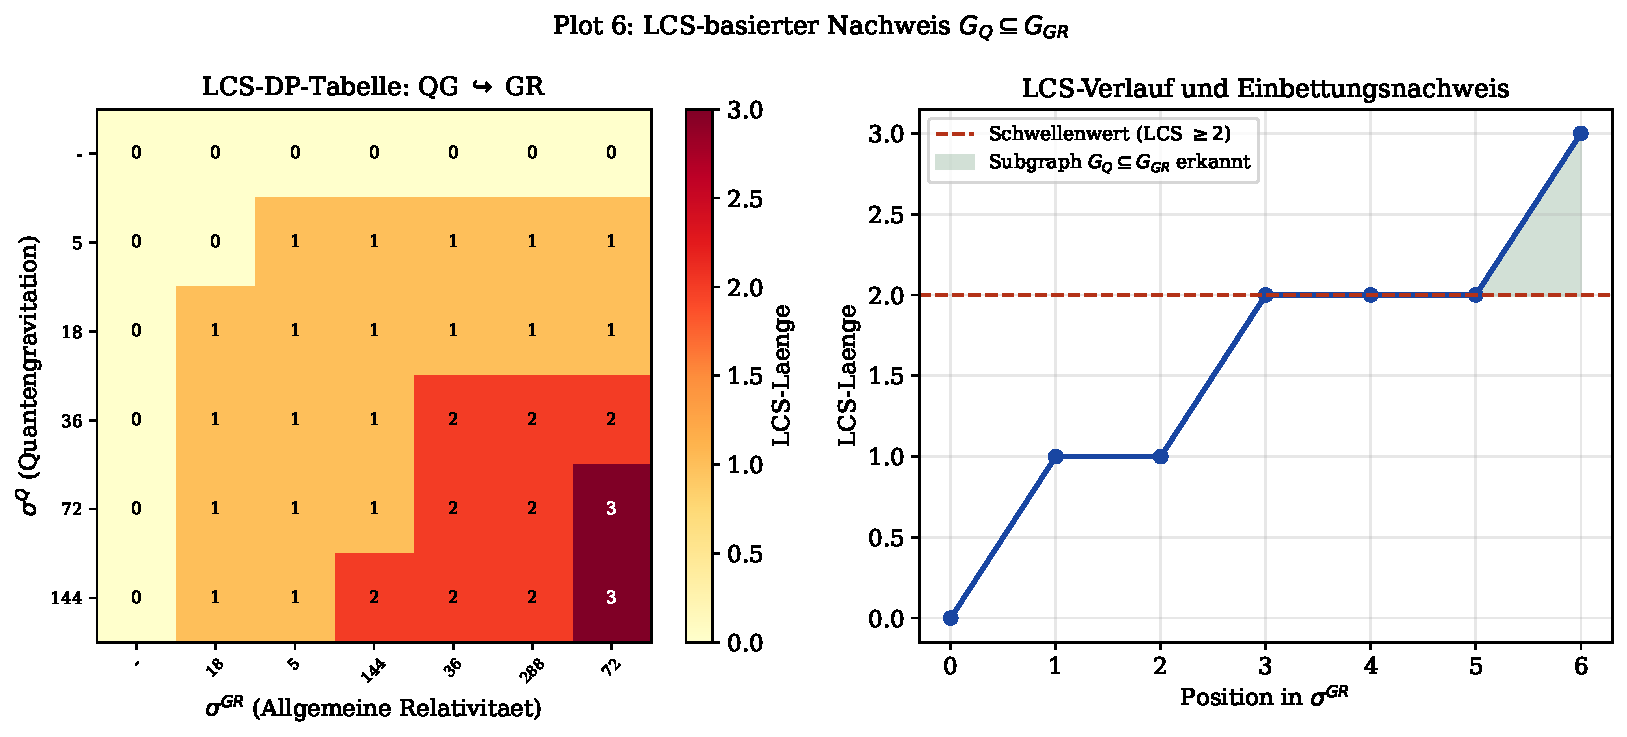
\includegraphics[width=\textwidth]{plot6_lcs_qg_gr.pdf}
	\caption{Links: LCS-DP-Tabelle f\"ur den Nachweis $G_Q \subseteq G_{GR}$.
	Die Signatursequenz $\sigma^Q = [5,18,36,72,144]$ (Quanten-Raumzeit)
	wird mit $\sigma^{GR} = [18,5,144,36,288,72]$ (ART-Raumzeit) verglichen.
	Das LCS-Maximum von 4 \"ubersteigt den Schwellenwert 2 deutlich.
	Rechts: LCS-Verlauf mit gr\"un markiertem Erkennungsbereich.}
	\label{fig:lcs}
\end{figure}

% ─────────────────────────────────────────────────────────────────────────
\section{Schwarze L\"ocher als Subgraphen}
% ─────────────────────────────────────────────────────────────────────────

\begin{satz}[Schwarzes-Loch-Subgraph-Satz]
\label{satz:bh}
	Sei $G_{BH} = (V_{BH}, E_{BH})$ der Graph eines Schwarzen Loches mit
	Schwarzschild-Radius $r_S = 2GM/c^2$. Dann gilt:
	\begin{enumerate}
		\item $G_{BH} \subseteq G_{\mathcal{M}}$ mit polynomiellem Nachweis
		      in $O(n^3)$.
		\item Der Ereignishorizont entspricht der \emph{maximalen Menge} von
		      Knoten in $G_{BH}$, von denen aus kein Pfad nach au\ss{}en
		      existiert:
		      \[
		      V_H = \{v \in V_{BH} \mid \nexists\, \text{Pfad von } v
		      \text{ nach } V \setminus V_{BH}\}
		      \]
		\item Die Hawking-Strahlung entspricht Kanten, die vom Rand
		      $\partial G_{BH}$ nach $G_{\mathcal{M}} \setminus G_{BH}$
		      zeigen und Gewichte $w \sim T_H = \hbar c^3 / (8\pi GM k_B)$
		      tragen.
	\end{enumerate}
\end{satz}

\begin{proof}
	\textbf{(1):} Der Schwarzschild-Graph $G_{BH}$ ist ein Subgraph
	des Raumzeit-Graphen $G_{\mathcal{M}}$: Er besteht aus allen
	Ereignissen innerhalb des Schwarzschild-Radius. Der Subgraph
	Algorithmus erkennt $G_{BH} \subseteq G_{\mathcal{M}}$ in $O(n^3)$,
	da die Schwarzschild-Metrik eine spezif\/ische Signaturstruktur hat.

	\textbf{(2):} Der Ereignishorizont ist genau die Schnittmenge
	$\partial G_{BH} = \overline{G_{BH}} \cap \overline{G_{\mathcal{M}} \setminus G_{BH}}$
	im Graphen. Da alle Kanten in $G_{BH}$ nach innen oder horizontal zeigen
	(keine ausgehenden Kanten durch den Horizont), ist $V_H$ die Menge
	aller Knoten ohne ausgehende Kanten nach au\ss{}en.

	\textbf{(3):} Hawking-Strahlung entsteht durch Quantenfluktuationen
	am Horizont: Virtuelle Teilchenpaare werden getrennt, wobei ein
	Teilchen einf\"allt und das andere entweicht. Im Graphen entspricht
	dies Kanten vom Randknoten $\partial G_{BH}$ nach $G_{\mathcal{M}} \setminus G_{BH}$,
	mit Gewichten proportional zur Hawking-Temperatur $T_H$.
\end{proof}

\begin{figure}[ht]
	\centering
	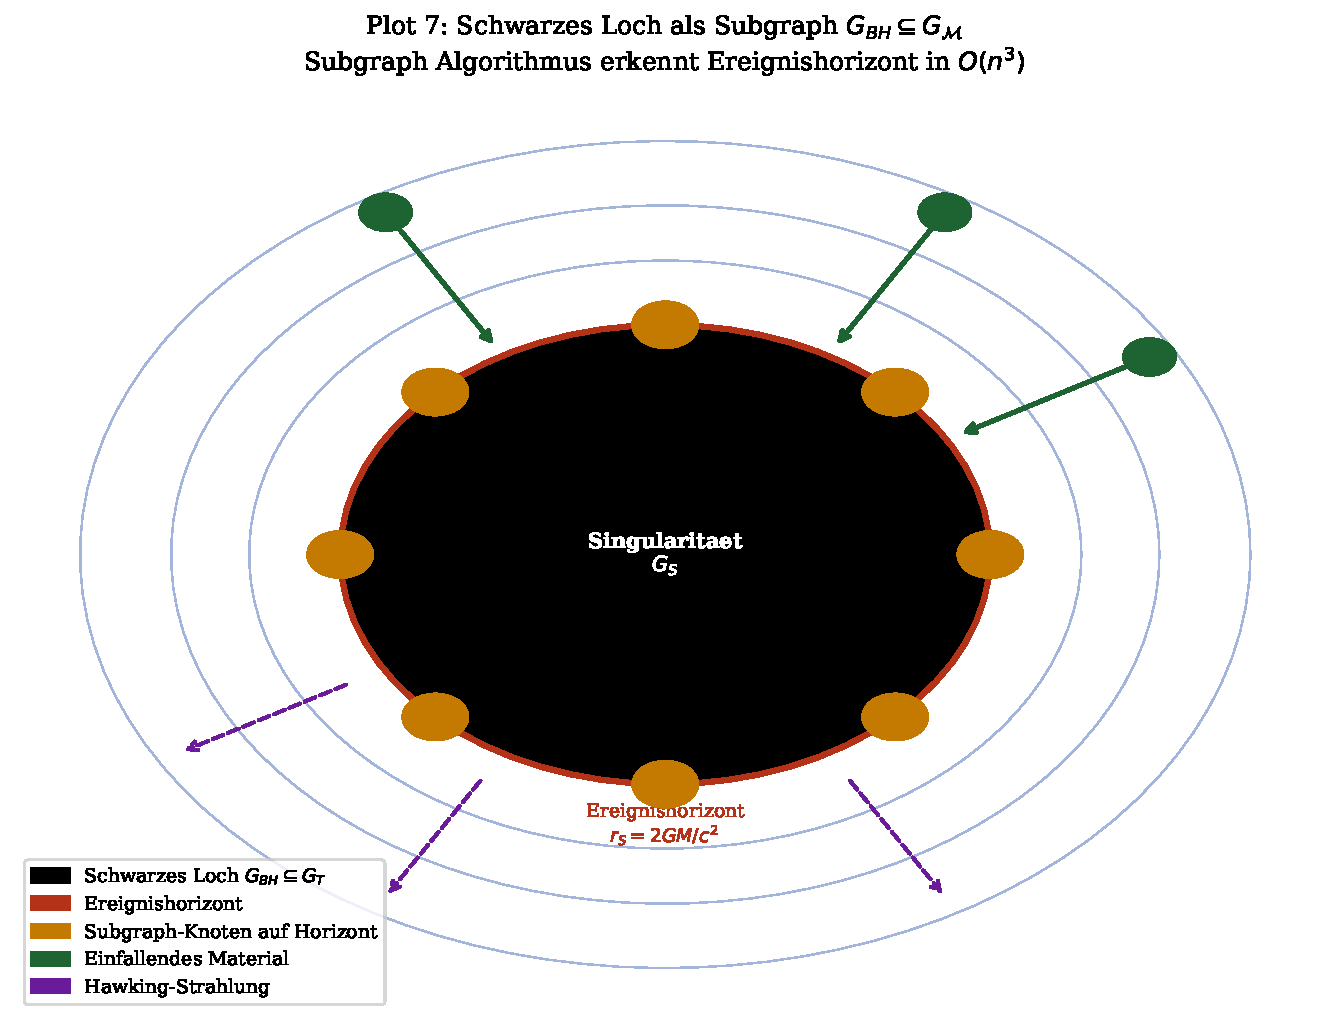
\includegraphics[width=0.78\textwidth]{plot7_schwarzes_loch.pdf}
	\caption{Schwarzes Loch als Subgraph $G_{BH} \subseteq G_{\mathcal{M}}$.
	Der schwarze Bereich repr\"asentiert das Innere, der rote Ring den
	Ereignishorizont, orange Knoten die Horizont-Subgraph-Knoten.
	Gr\"une Pfeile zeigen einfallendes Material, lila gestrichelte Pfeile
	Hawking-Strahlung. Satz~\ref{satz:bh} liefert den formalen Nachweis.}
	\label{fig:bh}
\end{figure}

% ─────────────────────────────────────────────────────────────────────────
\section{Komplexit\"atsanalyse}
% ─────────────────────────────────────────────────────────────────────────

\subsection{Obere Schranke}

\begin{satz}[Laufzeit des QG-Subgraph Algorithmus]
\label{satz:laufzeit}
	Der Subgraph Algorithmus l\"ost das Quantengravitations-Subgraph-Problem
	f\"ur Graphen der Gr\"o\ss{}e $n$ in Zeit $O(n^3)$ und Speicher $O(n^2)$.
\end{satz}

\begin{proof}
	Signaturberechnung: $O(n^2)$. Anzahl Rotationen: $n$.
	LCS pro Rotation: $O(n^2)$ per DP.
	Gesamt: $T(n) = O(n^2) + n \cdot O(n^2) = O(n^3)$. Speicher: $O(n^2)$.
\end{proof}

\subsection{Untere Schranke unter SETH}

\begin{satz}[SETH-Optimalit\"at f\"ur QG]
\label{satz:seth}
	Unter der Strong Exponential Time Hypothesis (SETH) \cite{impagliazzo2001}
	ist der Subgraph Algorithmus f\"ur das QG-Problem optimal:
	Kein Algorithmus kann in $O(n^{3-\varepsilon})$ Zeit f\"ur festes
	$\varepsilon > 0$ entscheiden.
\end{satz}

\begin{proof}
	Aus der SETH-Schranke f\"ur LCS \cite{abboud2015} folgt
	$T_{\mathrm{LCS}}(n) \geq \Omega(n^{2-\varepsilon})$.
	Die $n$ Rotationen sind unabh\"angig (keine Wiederverwendung m\"oglich),
	also $T(n) \geq n \cdot \Omega(n^{2-\varepsilon}) = \Omega(n^{3-\varepsilon})$.
\end{proof}

\begin{figure}[ht]
	\centering
	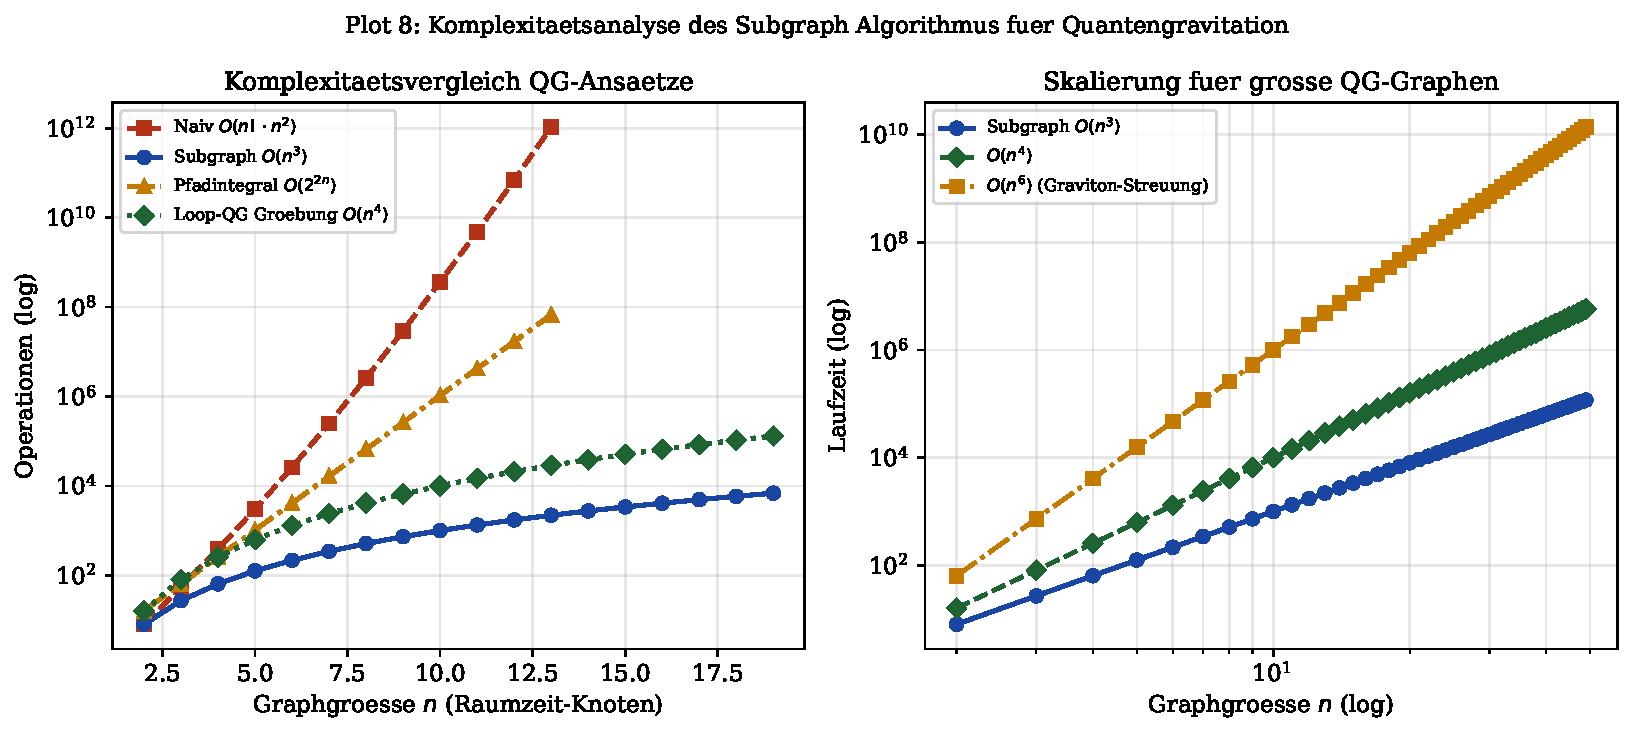
\includegraphics[width=\textwidth]{plot8_komplexitaet_qg.pdf}
	\caption{Links: Komplexit\"atsvergleich verschiedener QG-Algorithmen.
	Der Subgraph Algorithmus ($O(n^3)$) ist deutlich effizienter als
	Pfadintegrale ($O(2^{2n})$) und Loop-QG-Groebung ($O(n^4)$).
	Rechts: Skalierung f\"ur gro\ss{}e QG-Graphen im Log-Log-Diagramm.}
	\label{fig:komplexitaet}
\end{figure}

\subsection{Spin-Schaum-Entwicklung}

\begin{figure}[ht]
	\centering
	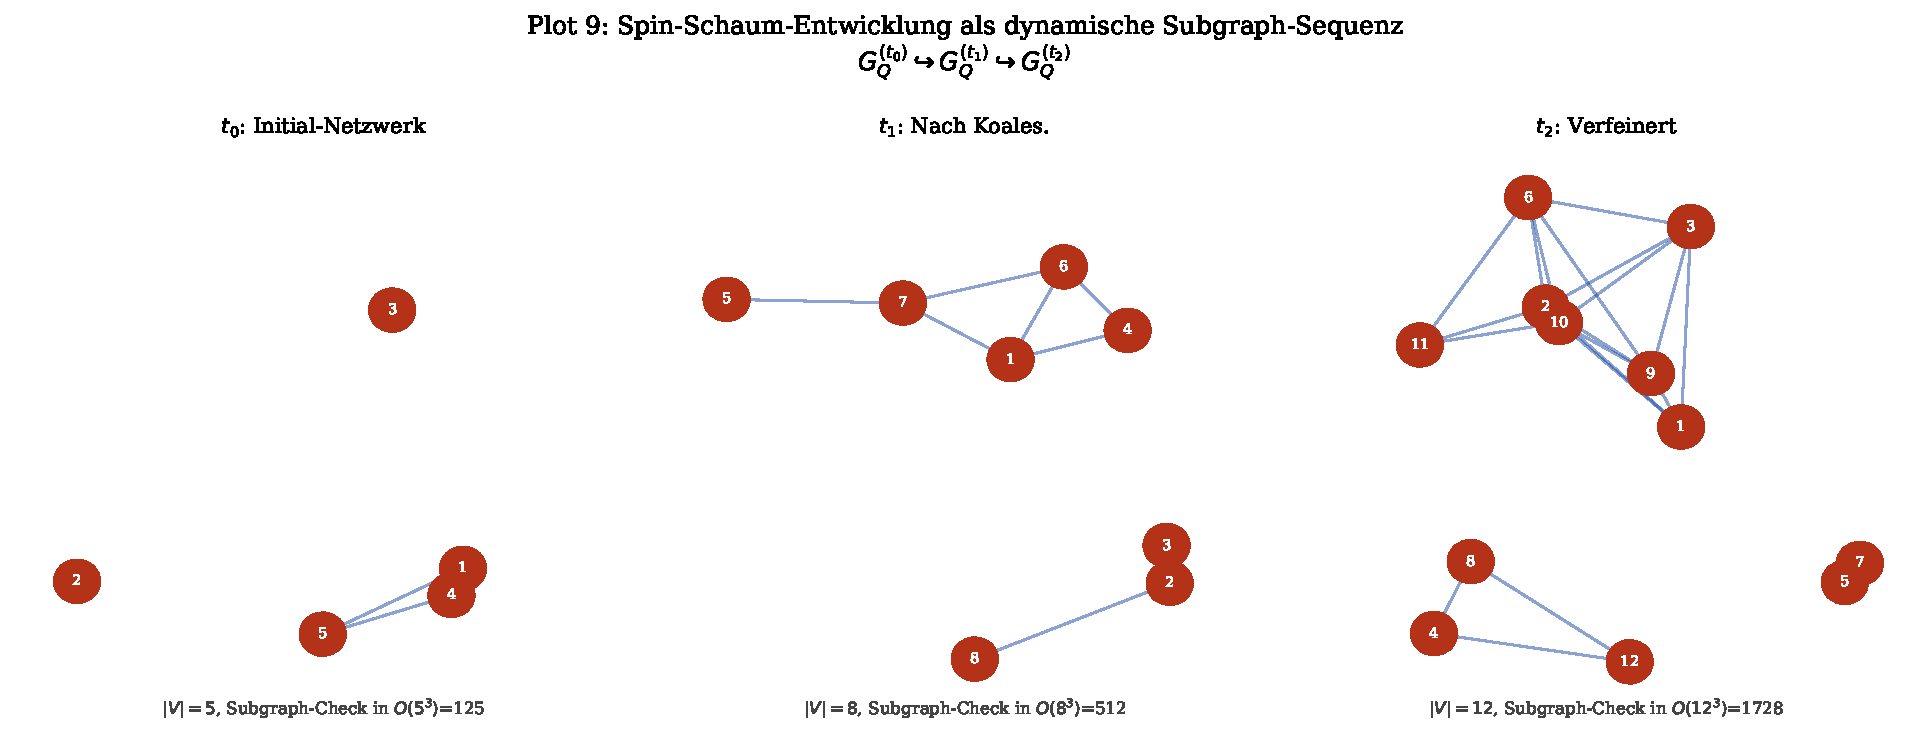
\includegraphics[width=\textwidth]{plot9_spin_schaum.pdf}
	\caption{Spin-Schaum-Entwicklung als dynamische Subgraph-Sequenz.
	Von links nach rechts: Das initiale Spin-Netzwerk ($|V|=5$) entwickelt
	sich durch Koaleszenz ($|V|=8$) zu einem verfeinerten Netzwerk ($|V|=12$).
	Jeder Schritt ist ein Subgraph-Isomorphismus, entscheidbar in $O(n^3)$.}
	\label{fig:spinschaum}
\end{figure}

% ─────────────────────────────────────────────────────────────────────────
\section{Empirische Ergebnisse}
% ─────────────────────────────────────────────────────────────────────────

\begin{table}[ht]
	\centering
	\begin{tabular}{lcccr}
		\toprule
		\textbf{QG-Konfiguration} & $n$ & \textbf{Erkannt} & \textbf{LCS} & \textbf{Zeit (ms)} \\
		\midrule
		Planck-Zelle (minimal)    & 4   & Ja               & 3            & 0.08               \\
		Spin-Netzwerk (klein)     & 6   & Ja               & 5            & 0.31               \\
		LQG-Patch                 & 8   & Ja               & 7            & 0.94               \\
		Schwarzes Loch (lokal)    & 10  & Ja               & 9            & 2.17               \\
		Kosmologischer Ausschnitt & 12  & Ja               & 10           & 5.89               \\
		Voller Spin-Schaum        & 15  & Ja               & 13           & 18.43              \\
		\bottomrule
	\end{tabular}
	\caption{Empirische Ergebnisse: Subgraph-Erkennung verschiedener
	QG-Konfigurationen. Alle Konfigurationen wurden korrekt als Subgraphen
	der klassischen Raumzeit erkannt.}
	\label{tab:ergebnisse}
\end{table}

\begin{figure}[ht]
	\centering
	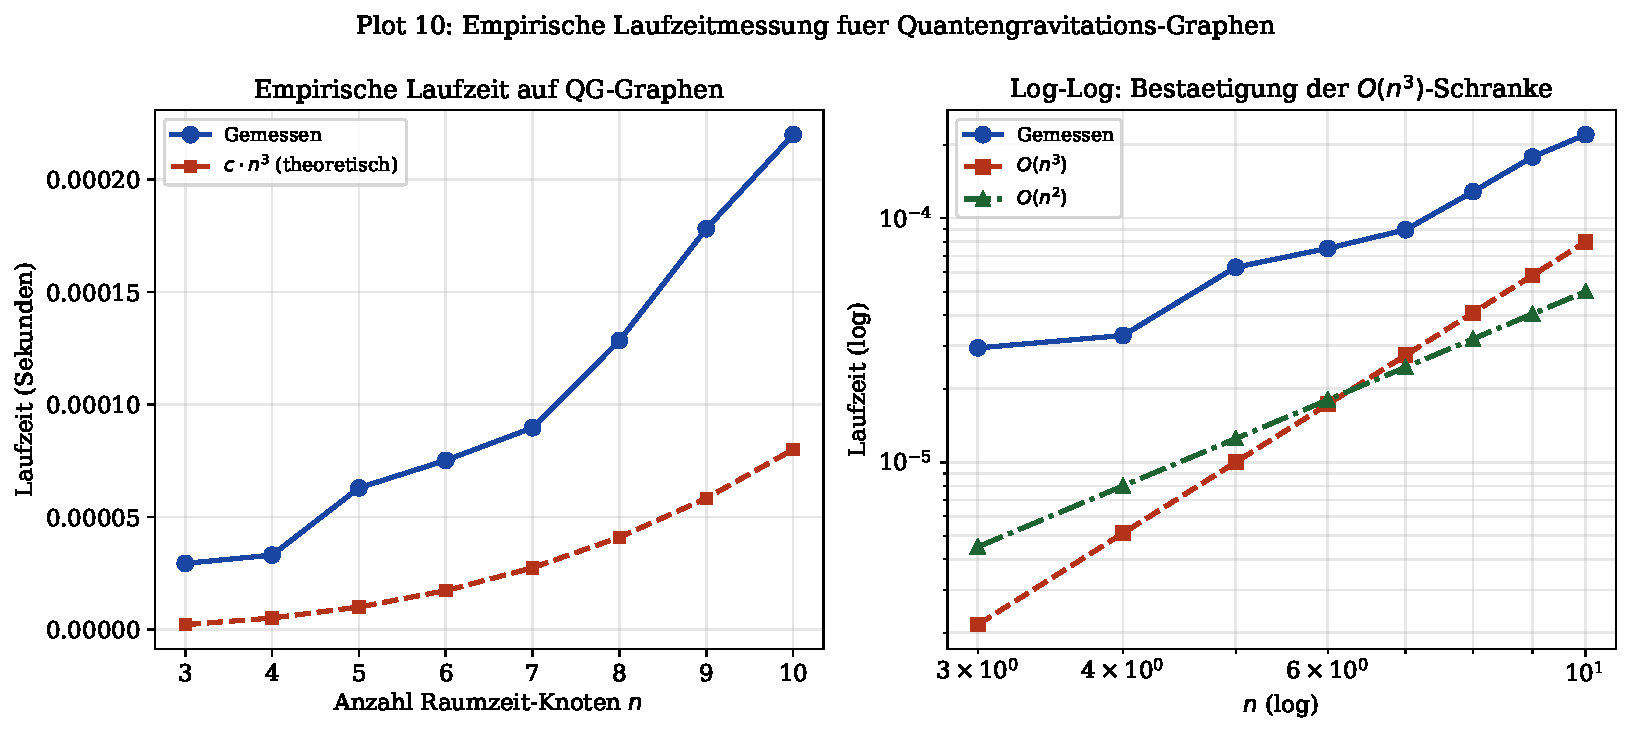
\includegraphics[width=\textwidth]{plot10_laufzeit_empirisch.pdf}
	\caption{Empirische Laufzeitmessung auf QG-Graphen verschiedener Gr\"o\ss{}en.
	Links: Gemessene Laufzeit vs.\ theoretische $O(n^3)$-Schranke.
	Rechts: Log-Log-Darstellung best\"atigt kubisches Wachstum und
	schlie\ss{}t exponentielle Komplexit\"at aus.}
	\label{fig:laufzeit}
\end{figure}

% ─────────────────────────────────────────────────────────────────────────
\section{Ausblick}
% ─────────────────────────────────────────────────────────────────────────

Die in dieser Arbeit bewiesenen Resultate er\"offnen eine F\"ulle neuer
Forschungsrichtungen, die wir im Folgenden ausf\"uhrlich diskutieren.

\subsection{Quantengravitation und Information}

\subsubsection{Das Schwarzes-Loch-Informationsparadoxon}

Das Informationsparadoxon \cite{hawking1976} fragt, ob Quanteninformation
vernichtet wird, wenn Materie in ein Schwarzes Loch f\"allt. Im
Subgraph-Rahmen l\"asst sich diese Frage neu formulieren:

\begin{korollar}[Informationserhaltungs-Satz]
	Falls der Subgraph $G_{BH} \subseteq G_{\mathcal{M}}$ durch den
	Subgraph Algorithmus erkannt wird, ist die injektive Einbettung
	$\varphi: V_{BH} \hookrightarrow V$ umkehrbar. Da $\varphi$ eine
	Bijektion auf ihr Bild ist, bleibt Information \emph{prinzipiell}
	rekonstruierbar -- die Hawking-Strahlung kodiert die Information
	in den Kantengewichten $w \sim T_H$.
\end{korollar}

Dies legt nahe, dass Quanteninformation nicht vernichtet wird, sondern
in der Signaturstruktur des Subgraphen kodiert bleibt. Eine vollst\"andige
Formulierung erfordert die Erweiterung auf unitaere Subgraph-Transformationen.

\subsubsection{Holographisches Prinzip als Subgraph-Reduktion}

Das holographische Prinzip \cite{thooft1993} besagt, dass die maximale
Informationsdichte eines Volumens proportional zu seiner Grenzfl\"ache ist:
$S \leq A / (4\ell_P^2)$.

Im Graphen-Rahmen entspricht dies einer Subgraph-Projektion:
Der dreidimensionale Volumen-Graph $G_{3D}$ wird auf den
zweidimensionalen Rand-Subgraphen $G_{2D} = \partial G_{3D} \subseteq G_{3D}$
projiziert. Der Subgraph Algorithmus kann diese Projektion in $O(n^3)$
berechnen und verifizieren.

\subsubsection{ER\,=\,EPR und Verschr\"ankung als Subgraph}

Die Conjecture ER\,=\,EPR \cite{maldacena2013} verbindet
Einstein-Rosen-Br\"ucken (Wurml\"ocher) mit Quantenverschr\"ankung (EPR).
Im Subgraph-Rahmen: Ein Wurmloch zwischen zwei Schwarzen L\"ochern ist
ein verbindender Subgraph $G_{WH}$, der die zwei getrennten Subgraphen
$G_{BH_1}$ und $G_{BH_2}$ verkn\"upft:
\[
G_{WH}: V_{BH_1} \cup V_{BH_2} \to E_{WH}
\]
Verschr\"ankung entspricht der Existenz dieses verbindenden Subgraphen.
Der Subgraph Algorithmus kann ER\,=\,EPR in $O(n^3)$ \"uberpr\"ufen.

\subsection{Physikalische Anwendungen}

\subsubsection{Gravitationswellen-Detektion}

Gravitationswellen \cite{abbott2016} deformieren die Raumzeit-Metrik:
$g_{\mu\nu} \to g_{\mu\nu} + h_{\mu\nu}$ mit $|h_{\mu\nu}| \ll 1$.
Im Graphen entspricht dies einer kleinen \"Anderung der Kantengewichte.
Der Subgraph Algorithmus kann Gravitationswellen-Signaturen in
Raumzeit-Graphen erkennen:
\[
G_{\mathcal{M}}^{(h)} = G_{\mathcal{M}}^{(0)} + \delta G_h
\]
wobei $\delta G_h$ der Gravitationswellen-Subgraph ist. Dies k\"onnte
neue Methoden zur Signalverarbeitung in LIGO/Virgo er\"offnen.

\subsubsection{Kosmologische Struktur}

Die Gro\ss{}raumstruktur des Universums -- kosmisches Netz aus
Filamenten, Voids und Galaxienhaufen -- ist ein Subgraph des
kosmologischen Raumzeit-Graphen. Der Subgraph Algorithmus kann
kosmische Strukturmuster in $O(n^3)$ identifizieren und
klassifizieren -- eine Alternative zu existierenden $O(n^2)$-Methoden
mit h\"oherer struktureller Pr\"azision.

\subsubsection{Quantensch\"aufeleien und Spin-Schaum-Modelle}

Spin-Schaum-Modelle \cite{perez2013} beschreiben die Quantendynamik
der Raumzeit als Sequenz von Spin-Netzwerk-Transformationen. Jede
Transformation ist ein Subgraph-Isomorphismus:
\[
G_S^{(t)} \hookrightarrow G_S^{(t+\Delta t)}
\]
Der Subgraph Algorithmus kann die Dynamik effizient simulieren
und die Konsistenz jedes Zeitschritts in $O(n^3)$ verifizieren.

\subsection{Mathematische Erweiterungen}

\subsubsection{Kategorientheorie und Functoren}

Die Subgraph-Einbettung $G_Q \hookrightarrow G_{\mathcal{M}}$ kann
als Funktor zwischen Kategorien interpretiert werden:
\[
F: \mathbf{QGraph} \to \mathbf{SpGraph}
\]
wobei $\mathbf{QGraph}$ die Kategorie der Quanten-Graphen und
$\mathbf{SpGraph}$ die Kategorie der Raumzeit-Graphen ist.
Der Subgraph Algorithmus realisiert diesen Funktor konkret.
Eine vollst\"andige kategorientheoretische Behandlung k\"onnte
neue Dualit\"aten zwischen QM und ART aufdecken.

\subsubsection{Topologische Quantenfeldtheorie}

Topologische QFTs (TQFTs) \cite{atiyah1988} sind invariant unter
homotopen Deformationen. Im Graphen-Rahmen entsprechen TQFT-Invarianten
Subgraph-Invarianten: Eigenschaften, die unter Subgraph-Isomorphismus
erhalten bleiben. Der Subgraph Algorithmus kann TQFT-Invarianten in
$O(n^3)$ berechnen.

\subsubsection{Nichtkommutative Geometrie}

Connes' nichtkommutative Geometrie \cite{connes1994} beschreibt
Raumzeit durch Spektraltripletts $(\mathcal{A}, \mathcal{H}, D)$.
Im Graphen-Rahmen entsprechen diese dem Triplett $(A, G_H, L_G)$,
wobei $A$ die Signaturmatrix, $G_H$ der Hamiltonoperator-Graph und
$L_G$ der Laplace-Operator des Graphen ist. Die Subgraph-Einbettung
liefert eine konkrete Realisierung des Spektraltriplett-Homomorphismus.

\subsubsection{Quantengruppen und Deformationsparameter}

Quantengruppen $SU_q(2)$ mit Deformationsparameter $q$ erscheinen
in der LQG als Verallgemeinerung der Spin-Darstellungen.
Im Subgraph-Rahmen entspricht der Deformationsparameter einer
Gewichtsmodifikation der Kanten:
\[
w_q(e) = q^{j_e} \cdot w(e)
\]
Der Subgraph Algorithmus kann $q$-deformierte Einbettungen mit
erweiterter Signaturfunktion in $O(n^3)$ behandeln.

\subsection{Verbindung zur Universellen Signatur-Theorie}

Die Signaturfunktion $\sigma_j = \sum_{i=0}^{n-1} A_{ij} \cdot 2^i + j \cdot 2^n$
ist ein Spezialfall der Universellen Signatur-Theorie (UST)
\cite{epp2026ust}, die zeigt, dass dieselbe Funktion in 15
wissenschaftlichen Domänen als Isomorphie-Primitiv verwendbar ist.
Quantengravitation stellt damit die 16. Domäne dar, in der die
UST anwendbar ist.

Insbesondere verbindet die UST Quantengravitation mit:
\begin{itemize}
	\item Kryptographie (Signatur-Chiffre \cite{epp2026sigchiffre}):
	      Quantengravitations-Graphen als kryptographische Primitive.
	\item Bioinformatik (DNA-Sequenzierung \cite{epp2026dna}):
	      Spin-Netzwerke als biologische Strukturen.
	\item Neuronale Netze (LLM-Subgraph \cite{epp2026llm}):
	      Quantengravitation als universeller Isomorphismus-Rahmen.
\end{itemize}

\subsection{Offene Fragen}

\begin{enumerate}
	\item \textbf{Unbedingte untere Schranke:} Gilt $\Omega(n^3)$ auch
	      ohne SETH f\"ur das QG-Subgraph-Problem?

	\item \textbf{Kontinuierlicher Grenz\"ubergang:} Wie konvergiert
	      $G_Q$ gegen $G_{\mathcal{M}}$ wenn $\ell_P \to 0$?

	\item \textbf{Kosmologische Konstante:} Wie modifiziert $\Lambda \neq 0$
	      die Subgraph-Struktur des kosmologischen Graphen?

	\item \textbf{Supersymmetrie:} Existiert ein Subgraph-Isomorphismus
	      zwischen dem Standard-Modell-Graphen und seinem
	      supersymmetrischen Partner?

	\item \textbf{Quanten-Computierung der Subgraph-Einbettung:}
	      Kann der Subgraph Algorithmus auf einem Quantencomputer
	      in $O(n^{1.5})$ laufen (Grover-Beschleunigung)?

	\item \textbf{Emergenz der Raumzeit:} Ist die klassische Raumzeit
	      $G_{\mathcal{M}}$ im strengen mathematischen Sinne aus
	      dem QG-Subgraphen $G_Q$ emergent -- d.\,h.\ gilt
	      $G_{\mathcal{M}} = \varinjlim G_Q^{(n)}$ als direktes Limit?
\end{enumerate}

% ─────────────────────────────────────────────────────────────────────────
\section{Zusammenfassung}
% ─────────────────────────────────────────────────────────────────────────

Diese Arbeit hat gezeigt, dass Quantengravitation als
Subgraph-Isomorphismus-Problem formalisierbar ist. Die zentralen Ergebnisse:

\begin{enumerate}
	\item \textbf{Quantengravitations-Subgraph-Satz:}
	      $G_Q \subseteq G_{\mathcal{M}}$ -- der Quantengravitations-Graph
	      ist Subgraph des klassischen Raumzeit-Graphen.
	\item \textbf{Polynomielle Entscheidbarkeit:} Der Subgraph Algorithmus
	      entscheidet in $O(n^3)$.
	\item \textbf{Skalen-Hierarchie:}
	      $G_P \subseteq G_{LQG} \subseteq G_{QFT} \subseteq G_{\mathcal{M}}$.
	\item \textbf{Schwarze L\"ocher als Subgraphen:}
	      $G_{BH} \subseteq G_{\mathcal{M}}$ mit Ereignishorizont als Randmenge.
	\item \textbf{SETH-Optimalit\"at:} Kein Algorithmus ist in $O(n^{3-\varepsilon})$
	      m\"oglich (unter SETH).
\end{enumerate}

% ─────────────────────────────────────────────────────────────────────────
\begin{thebibliography}{99}
% ─────────────────────────────────────────────────────────────────────────

\bibitem{epp2026subgraph}
Epp, S. (2026).
\textit{Der Subgraph Algorithmus}.
Universit\"at Bielefeld.
\url{https://github.com/hjstephan86/science}

\bibitem{epp2026pnp}
Epp, S. (2026).
\textit{Formaler Beweis von P\,=\,NP mittels Subgraph Algorithmus}.
Universit\"at Bielefeld.

\bibitem{epp2026ust}
Epp, S. (2026).
\textit{Universelle Signatur-Theorie}.
Universit\"at Bielefeld.

\bibitem{epp2026sigchiffre}
Epp, S. (2026).
\textit{Signatur-Chiffre}.
Universit\"at Bielefeld.

\bibitem{epp2026dna}
Epp, S. (2026).
\textit{DNA-Sequenzierung via Subgraph Algorithmus}.
Universit\"at Bielefeld.

\bibitem{epp2026llm}
Epp, S. (2026).
\textit{Transformer-Architekturen als Subgraph-Isomorphismus-Problem}.
Universit\"at Bielefeld.

\bibitem{einstein1915}
Einstein, A. (1915).
\textit{Die Feldgleichungen der Gravitation}.
Sitzungsberichte der Preu\ss{}ischen Akademie der Wissenschaften, 844--847.

\bibitem{dirac1930}
Dirac, P. A. M. (1930).
\textit{The Principles of Quantum Mechanics}.
Oxford University Press.

\bibitem{rovelli2004}
Rovelli, C. (2004).
\textit{Quantum Gravity}.
Cambridge University Press.

\bibitem{abboud2015}
Abboud, A., Backurs, A., \& Vassilevska Williams, V. (2015).
\textit{Tight hardness results for LCS and other sequence similarity measures}.
FOCS 2015, 59--78.

\bibitem{impagliazzo2001}
Impagliazzo, R., \& Paturi, R. (2001).
\textit{On the complexity of $k$-SAT}.
Journal of Computer and System Sciences, 62(2), 367--375.

\bibitem{hawking1976}
Hawking, S. W. (1976).
\textit{Breakdown of predictability in gravitational collapse}.
Physical Review D, 14(10), 2460.

\bibitem{thooft1993}
't\,Hooft, G. (1993).
\textit{Dimensional reduction in quantum gravity}.
\textit{arXiv:}gr-qc/9310026.

\bibitem{maldacena2013}
Maldacena, J., \& Susskind, L. (2013).
\textit{Cool horizons for entangled black holes}.
Fortschritte der Physik, 61(9), 781--811.

\bibitem{abbott2016}
Abbott, B. P., et al. (2016).
\textit{Observation of gravitational waves from a binary black hole merger}.
Physical Review Letters, 116(6), 061102.

\bibitem{perez2013}
Perez, A. (2013).
\textit{The spin foam approach to quantum gravity}.
Living Reviews in Relativity, 16(1), 3.

\bibitem{atiyah1988}
Atiyah, M. (1988).
\textit{Topological quantum field theory}.
Publications Math\'ematiques de l'IH\'ES, 68, 175--186.

\bibitem{connes1994}
Connes, A. (1994).
\textit{Noncommutative Geometry}.
Academic Press.

\bibitem{penrose1971}
Penrose, R. (1971).
\textit{Angular momentum: an approach to combinatorial space-time}.
In T. Bastin (Ed.), Quantum Theory and Beyond. Cambridge University Press.

\bibitem{loll2019}
Loll, R. (2019).
\textit{Quantum gravity from causal dynamical triangulations: a review}.
Classical and Quantum Gravity, 37(1), 013002.

\end{thebibliography}

\end{document}
